%%%%%%%%%%%%%%%%%%%%%%%%%%%%%%%%%%%%%%%%%
% Arsclassica Article
% LaTeX Template
% Version 1.0 (21/4/14)
%
% This template has been downloaded from:
% http://www.LaTeXTemplates.com
%
% Original author:
% Lorenzo Pantieri (http://www.lorenzopantieri.net) with extensive modifications by:
% Vel (vel@latextemplates.com)
%
% License:
% CC BY-NC-SA 3.0 (http://creativecommons.org/licenses/by-nc-sa/3.0/)
%
%%%%%%%%%%%%%%%%%%%%%%%%%%%%%%%%%%%%%%%%%

%----------------------------------------------------------------------------------------
%	PACKAGES AND OTHER DOCUMENT CONFIGURATIONS
%----------------------------------------------------------------------------------------
\documentclass[
10pt, % Main document font size
a4paper, % Paper type, use 'letterpaper' for US Letter paper
oneside, % One page layout (no page indentation)
%twoside, % Two page layout (page indentation for binding and different headers)
headinclude,footinclude, % Extra spacing for the header and footer
BCOR5mm, % Binding correction
]{scrartcl}


%%%%%%%%%%%%%%%%%%%%%%%%%%%%%%%%%%%%%%%%%
% Arsclassica Article
% Structure Specification File
%
% This file has been downloaded from:
% http://www.LaTeXTemplates.com
%
% Original author:
% Lorenzo Pantieri (http://www.lorenzopantieri.net) with extensive modifications by:
% Vel (vel@latextemplates.com)
%
% License:
% CC BY-NC-SA 3.0 (http://creativecommons.org/licenses/by-nc-sa/3.0/)
%
%%%%%%%%%%%%%%%%%%%%%%%%%%%%%%%%%%%%%%%%%

%----------------------------------------------------------------------------------------
%	REQUIRED PACKAGES
%----------------------------------------------------------------------------------------

\usepackage[
nochapters, % Turn off chapters since this is an article        
beramono, % Use the Bera Mono font for monospaced text (\texttt)
eulermath,% Use the Euler font for mathematics
pdfspacing, % Makes use of pdftex’ letter spacing capabilities via the microtype package
dottedtoc % Dotted lines leading to the page numbers in the table of contents
]{classicthesis} % The layout is based on the Classic Thesis style

\usepackage{arsclassica} % Modifies the Classic Thesis package

\usepackage[T1]{fontenc} % Use 8-bit encoding that has 256 glyphs

\usepackage[utf8]{inputenc} % Required for including letters with accents

\usepackage{graphicx} % Required for including images
\graphicspath{{Figures/}} % Set the default folder for images

\usepackage{enumitem} % Required for manipulating the whitespace between and within lists

\usepackage{lipsum} % Used for inserting dummy 'Lorem ipsum' text into the template

\usepackage{subfig} % Required for creating figures with multiple parts (subfigures)

\usepackage{amsmath,amssymb,amsthm} % For including math equations, theorems, symbols, etc

\usepackage{varioref} % More descriptive referencing


%----------------------------------------------------------------------------------------
%	THEOREM STYLES
%---------------------------------------------------------------------------------------

\theoremstyle{definition} % Define theorem styles here based on the definition style (used for definitions and examples)
\newtheorem{definition}{Definition}

\theoremstyle{plain} % Define theorem styles here based on the plain style (used for theorems, lemmas, propositions)
\newtheorem{theorem}{Theorem}

\theoremstyle{remark} % Define theorem styles here based on the remark style (used for remarks and notes)

%----------------------------------------------------------------------------------------
%	HYPERLINKS
%---------------------------------------------------------------------------------------

\hypersetup{
%draft, % Uncomment to remove all links (useful for printing in black and white)
colorlinks=true, breaklinks=true, bookmarks=true,bookmarksnumbered,
urlcolor=webbrown, linkcolor=RoyalBlue, citecolor=webgreen, % Link colors
pdftitle={}, % PDF title
pdfauthor={\textcopyright}, % PDF Author
pdfsubject={}, % PDF Subject
pdfkeywords={}, % PDF Keywords
pdfcreator={pdfLaTeX}, % PDF Creator
pdfproducer={LaTeX with hyperref and ClassicThesis} % PDF producer
} % Include the structure.tex file which specified the document structure and layout
\usepackage{verbatim}
\hyphenation{Fortran hy-phen-ation} % Specify custom hyphenation points in words with dashes where you would like hyphenation to occur, or alternatively, don't put any dashes in a word to stop hyphenation altogether

%----------------------------------------------------------------------------------------
%	TITLE AND AUTHOR(S)
%----------------------------------------------------------------------------------------

\title{\normalfont\spacedallcaps{Sub-Jupiter Radius Occurrence Rate Anomaly}} % The article title

\author{\spacedlowsmallcaps{Joe Renaud}} % The article author(s) - author affiliations need to be specified in the AUTHOR AFFILIATIONS block

\date{} % An optional date to appear under the author(s)

%----------------------------------------------------------------------------------------

\begin{document}

%----------------------------------------------------------------------------------------
%	HEADERS
%----------------------------------------------------------------------------------------

\renewcommand{\sectionmark}[1]{\markright{\spacedlowsmallcaps{#1}}} % The header for all pages (oneside) or for even pages (twoside)
%\renewcommand{\subsectionmark}[1]{\markright{\thesubsection~#1}} % Uncomment when using the twoside option - this modifies the header on odd pages
\lehead{\mbox{\llap{\small\thepage\kern1em\color{halfgray} \vline}\color{halfgray}\hspace{0.5em}\rightmark\hfil}} % The header style

\pagestyle{scrheadings} % Enable the headers specified in this block

%----------------------------------------------------------------------------------------
%	TABLE OF CONTENTS & LISTS OF FIGURES AND TABLES
%----------------------------------------------------------------------------------------

\maketitle % Print the title/author/date block

\setcounter{tocdepth}{2} % Set the depth of the table of contents to show sections and subsections only

\tableofcontents % Print the table of contents

\listoffigures % Print the list of figures

\listoftables % Print the list of tables

%----------------------------------------------------------------------------------------
%	ABSTRACT
%----------------------------------------------------------------------------------------

\section*{Abstract} % This section will not appear in the table of contents due to the star (\section*)

%----------------------------------------------------------------------------------------
%	AUTHOR AFFILIATIONS
%----------------------------------------------------------------------------------------

%\let\thefootnote\relax\footnotetext{* \textit{Department of Biology, University of Examples, London, United Kingdom}}

%\let\thefootnote\relax\footnotetext{\textsuperscript{1} \textit{Department of Chemistry, University of Examples, London, United Kingdom}}

%----------------------------------------------------------------------------------------

\newpage % Start the article content on the second page, remove this if you have a longer abstract that goes onto the second page

%----------------------------------------------------------------------------------------
%	INTRODUCTION
%----------------------------------------------------------------------------------------

\section{Introduction}

Since the first confirmation of an extra-solar planet in 1992\cite{Wolszczan:1992}, the field of exoplanet research has exploded with nearly 1800 planets currently confirmed (as of May 6th, 2014\cite{ExoData:nasa}). Since the early 90's the detection techniques employed to discover these exoplanets relied heavily upon tracking the Doppler shift in a host star's spectrum. Such a shift could arise from a large, short period, exoplanet. The radial velocity technique formed the majority of exoplanet confirmations well into the late 2000's\cite{RV1}. During this time the transit technique started to gain prevalence. 
\subsection{Transit Technique and NASA's Kepler Mission}
Exoplanet transiting refers to the event when a exoplanet passes into the line of sight of the observer to the host star. A host star's light can be monitored over a certain time span; when compared to the light output of similar stars in the same frame - a exoplanet detection can be easily picked out (see figure~\vref{fig:transit}). These light curves allow researchers to determine certain characteristics of the transiting planet. Specifically from one transit one can find the ratio of the radius of the planet compared to the host star. Multiple transits will provide orbital information\cite{TR1}.
\begin{figure}[tb]
\centering 
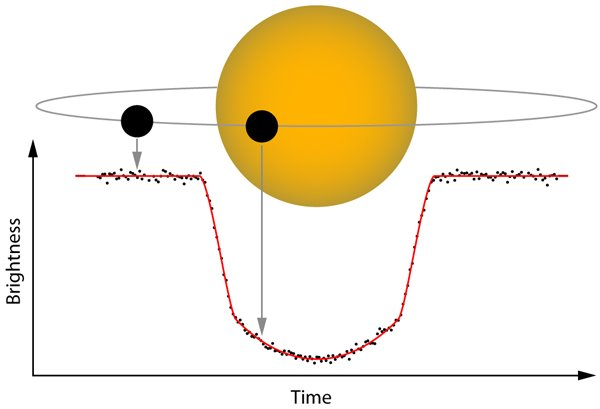
\includegraphics[width=0.5\columnwidth]{transit} 
\caption[Transiting Exoplanet]{Cartoon of a transiting exoplanet, image taken from NASA exoplanet database}
\label{fig:transit} 
\end{figure}
The early days of transit discoveries found only large radius planets as these required the least sensitive equipment, and from the fact that the signal to noise ratio of an exoplanet discovery is described by equations 1 and 2. 
\begin{equation}
\frac{S}{N} \approx \sqrt{N_{t}}\frac{\delta}{\sigma}
\label{eq:t1}
\end{equation}
\begin{equation}
\delta = \left(\frac{R_{p}}{R_{*}}\right)^{2}
\label{eq:t2}
\end{equation}
The radius of the planet $R_{p}$ and the radius of the star $R_{*}$ greatly impacts the S/N, as does the photometric precision $\sigma$\cite{DST}. Thus, these early discoveries had limited (and small) photometric precision. Therefore, the only planets that had a decent signal to noise ratio were those with large radii. This can be seen in the histogram of radii for all exoplanets discovered by the transit technique up to 2008 (Figure~\vref{fig:transit2}). Jupiter size planets and larger were common discoveries for the transit technique. It was not until NASA's Kepler mission was launched in 2009\cite{kep2} that photometric precision was increased to the point that sub-Jupiter planets could be detected\cite{kep1}. Once Kepler's data began getting published it became clear that not only could Kepler detect planets down to the sub-Earth size, but it was also able to find planets much more quickly - increasing the exoplanet database size dramatically (Figure~\vref{fig:transit2}). There are over 1700 exoplanets discovered through the transit, and other techniques (last checked on May 10th 2014\cite{ExoData:nasa}). All of these planets provide a good sampling of the potential exoplanets within our galaxy. There has been a number of studies that examine properties of the currently discovered exoplanets (e.g: \cite{occ1,Marcey1,occ2}). This project examines an anomaly in the distribution of exoplanet radii in transiting exoplanets.
\begin{figure}[tb]
\centering 
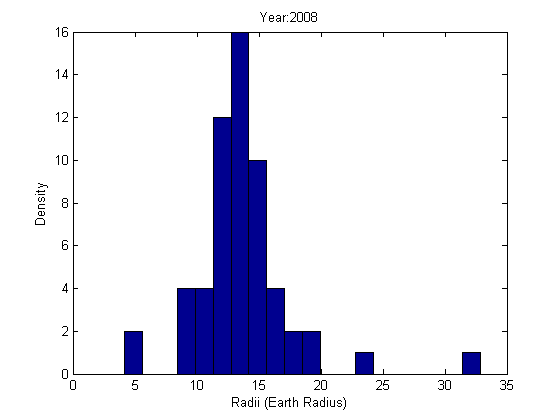
\includegraphics[width=0.8\columnwidth]{2008TransitRadius} 
\caption[>2008 Exoplanet transit discoveries]{Exoplanet discoveries made by the transiting technique from 1990 to 2008. The radii are measured in Earth Radii, with ~10 Earth Radius being roughly the size of Jupiter.}
\label{fig:transit2} 
\end{figure}
\begin{figure}[tb]
\centering 
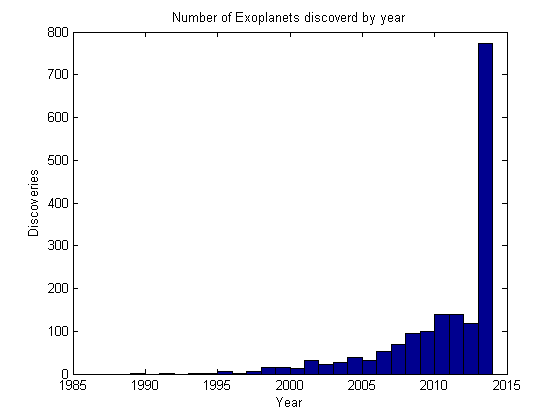
\includegraphics[width=0.8\columnwidth]{2014Transit} 
\caption[Current Transit Technique Discoveries]{Transit technique discoveries up to April 25th 2014. It is clear that since Kepler's launch in 2009, the exoplanet database has grown substantially.}
\label{fig:transit2} 
\end{figure}
\subsection{Radii of Discovered Planets}
We are specifically curious what the distribution of exoplanet radius has been changing since the introduction of the Kepler mission. Since radius is a primary variable of only the transit technique: most of the analysis will be based upon planets discovered by transiting. However, some planets originally discovered by radial velocity, or other techniques, have been reexamined by telescopes using the transit technique. This allows some analysis of radii of radial velocity exoplanets. 


 
%----------------------------------------------------------------------------------------
%	METHODS
%----------------------------------------------------------------------------------------
\subsection{Data}
The data for this study is obtained from \href{"http://exoplanetarchive.ipac.caltech.edu/cgi-bin/ExoTables/nph-exotbls?dataset=planets"}{NASA Confirmed Exoplanet Database} and 
\href{"http://exoplanetarchive.ipac.caltech.edu/cgi-bin/ExoTables/nph-exotbls?dataset=cumulative"}{NASA Exoplanet Candidate Database}. This data is updated continuously by the scientific community and managed by NASA, making it a very reliable source. The specific type of data that can be pulled from this source includes publication date, Planetary properties (mass, radius, period, etc), Stellar properties (mass, radius, galactic location, etc), and detection information. A number of planets detected by the transit method up to the current date can be found on figure~\vref{fig:transit2}. To ensure reliability of data: any exoplanet that was examined was first cross referenced on a different, but still well cited, exoplanet database - \href{"http://exoplanets.eu/"}{Exoplanets.eu}. Specifically, planet radii were confirmed to be the same across both databases. Any planet that had a significant variation across the sources was neglected from the study. 

Issues with this data is that the date listed does not necessarily correspond to the date when technology was sufficient enough to detect said planet, but rather when enough research and/or follow-ups were preformed to make a publication regarding its discovery. This means that the capability of discovering does not scale with publication year. This means that predictions as to when technology will be sufficient enough to detect a planet of a certain radius ( $P(R)\propto{}R^{n}$, for some n ) can not be easily extrapolated. This also means that the planets that show up in either of these databases will be dependent on where research times is being focused.
\subsection{Previous Work}
Exoplanet occurrence work has been done extensively in the past (\cite{pug,Marcey1,occ2,occ1}). These studies focus on the probability of finding certain characteristics in planets around stars. The methods to preform this are varied. However, several studies (\cite{occ2,pug,Marcey1}) focus on the total number of planets found with a certain characteristic (e.g: $R=1-1.5R_{E}$ ) and divide them by the total number of stars observed within that time-frame. Complexities arise when trying to also account for the the false positive (FPs) rate of the various observations. The methods to categorize FPs vary by study, but a detailed explanation can be found within \cite{pug}.
This study looks at the overall characteristics of planets discovered to date. Not many publications take a step back and look at the overall picture of discovered planets. The particular characteristic we are currently interested in is the distribution of exoplanet radii. 
\section{Analysis}
We investigate a extinction zone in exoplanet detections with a range of $R \approx (5 - 10) R_{E}$ . An initial signature of this extinction can be seen in figure~\vref{fig:exo2}
\begin{figure}[tb]
\centering 
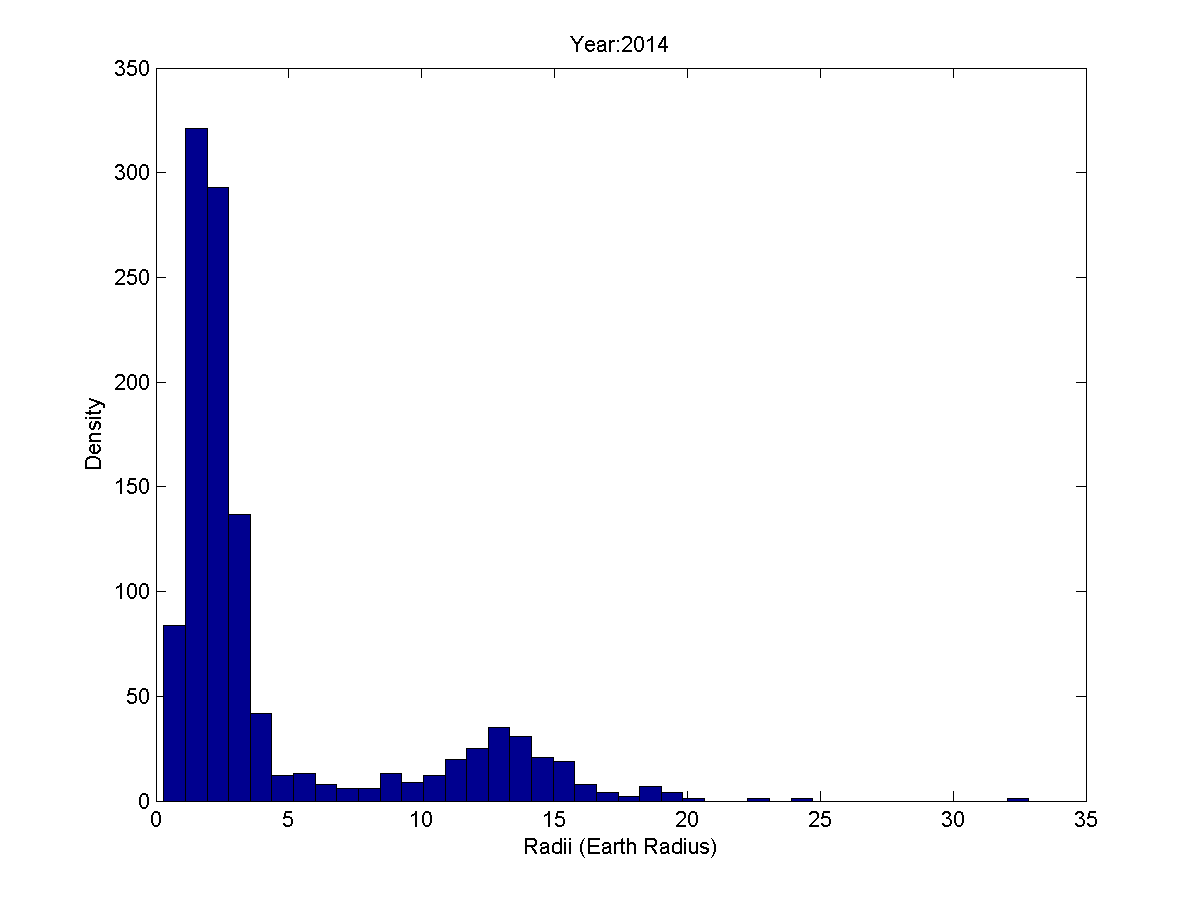
\includegraphics[width=0.8\columnwidth]{radi2014} 
\caption[Exoplanet Radii]{Histogram of Exoplanet radius from 1990 to May 10th, 2014. Detection techniques include transits, radial velocity, and other. The x-axis shows planet radius in units of Earth radii, the y-axis shows number of exoplanets with that radius. Specifically, note the extinction zone at $R \approx (5 - 10) R_{E}$ .}
\label{fig:exo2} 
\end{figure}
\subsection{Detection Analysis}
As previously mentioned, detection during the early years of exoplanet discoveries had a bias of detecting larger radius planets due to the signal to noise relationship (Eq.1). To compensate for this: data was examined using 2009 as a starting point. This indicates the last major technological advancement which had a significant affect on the signal to noise ratio (namely the launch of the Kepler spacecraft). The histogram of this data can be found in figure~\vref{fig:exo3}. Even though now we are looking at a time range that eliminates much of the original detection bias, we can still see a similar extinction zone as that seen in figure~\vref{fig:exo2}. Planets with $R=(10+) R_{E}$ are reduced compared to the previous plot. 
\begin{figure}[tb]
\centering 
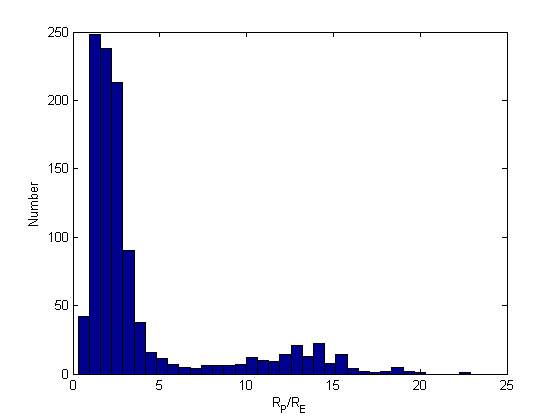
\includegraphics[width=0.8\columnwidth]{radi2009pl} 
\caption[Exoplanet Radii]{Histogram of Exoplanet radius from Jan 1st 2009 to May 10th, 2014. Detection techniques include transits, radial velocity, and other.}
\label{fig:exo3} 
\end{figure}
\subsection{Kepler Detection}
The next step is to determine which data is contributing to this extinction zone. Kepler data and non-Kepler data were examined against each other to see if there was an indication where the anomaly seen in figure~\vref{fig:exo3} originated from. The following expectations are expected, and seen in the results:
\begin{enumerate}
\item Non-Kepler data will not have a significant contribution for $R\lesssim{}9R_{E}$ . This is due to the poor sensitivity in all non-Kepler instruments. 
\item Kepler data is able to detect planets with $R \approx{} 1R_{E}$ . Thus, it will have a distribution proportionate to the actual radii distribution of observed star systems minus the false positive rate. 
\item Kepler data is expected to fall off quickly with $R < 1R_{E}$ . This is due to its own S/N ratio increasing at this point. There is also some arguments being made that planet formation will leave few objects around Mars radius to Earth Radius \cite{pug,Marcey1}. This is beyond the scope of this study.
\end{enumerate}
The comparison of these two data-sets can be seen in figure~\vref{fig:exocomp}. As expected we can see that the non-Kepler data has a sharp drop off at sub-Jupiter radius ( $10R_{E}$ ). However, the Kepler data shows a sharp drop off at $R\approx{}5R_{E}$. This is not expected as Kepler is capable of detecting larger planets as easily as non-Kepler instrumentation. The expected distribution would be decreasing at increasing R, but at a much slower rate. 
\begin{figure}[tb]
\centering 
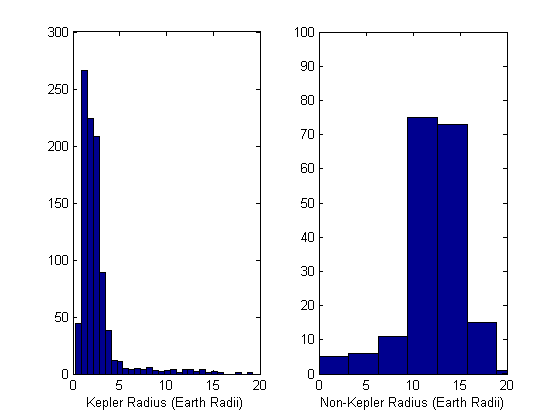
\includegraphics[width=0.8\columnwidth]{KepvNoKep} 
\caption[Kepler v. NonKepler]{Histograms of Exoplanet radius for Kepler and non-Kepler data from 2009 to May 10th, 2014.}
\label{fig:exocomp} 
\end{figure}
\subsection{Physical Explanations of Sub-Jupiter Radii Extinction}
Currently, all literature does not seem to predict a extinction of planets with radii between Super Earth and Sub-Jupiter. In fact \cite{pug} show that the probability should be continuously decreasing, with no bi-model behavior as seen in the actual data (see figure~\vref{fig:pug1}. An argument that is based in physical processes, instead of data, can be found in \cite{ray1} with similar conclusions.
\begin{figure}[tb]
\centering 
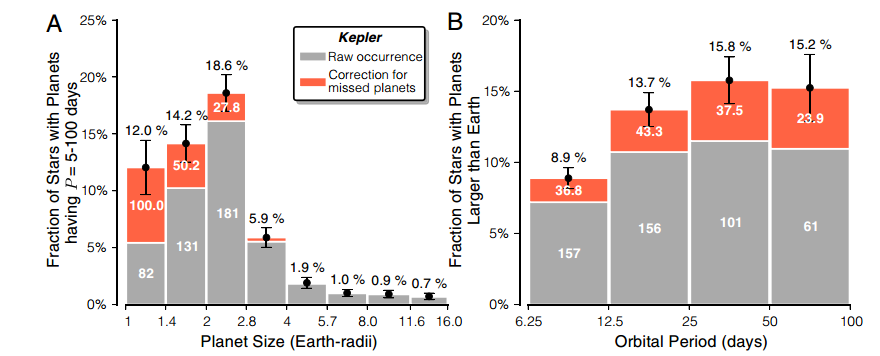
\includegraphics[width=1\columnwidth]{pug1} 
\caption[Probability of Star hosting Exoplanet with certain Radius]{Plot generated, and explained in depth, by Petigura et al \cite{pug}. The figure of interest is on the left: Probability of a star within the Kepler field of view hosting a planet of a certain radius.}
\label{fig:pug1} 
\end{figure}
\subsection{Confirmation of Significance and Possible Origin}
Since the databases we are parsing only show published exoplanets, then one possible explanation for the lack of confirmed planets around Neptune radii could be that Kepler data with $R > 5 R_{E}$ is not getting as much follow-up and research attention as those planets with $R < 5 R_{E}$. This is a difficult thing to test. However, the NASA exoplanet database does publish candidates which are not confirmed planets, but have some likely hood of confirmation. These candidates, by definition, have not received the required follow-ups or analysis to be classified as confirmed exoplanets. Generally, this means that Kepler has gathered strong light curve signatures, but not multiple ones (possibly due to long periods) or multiple ones that have indications of being false positives. These are legitimate problems for planets smaller than roughly 6 Earth radii, as other equipment is not sensitive enough to detect such planets. However, a sizable potion of planets within our area of interest are well within the precision of ground based observatories. Therefore, it is merely an issue of using those observatories to complete follow-ups on such planets. To show this we look at Kepler Candidates and Kepler Transit Events~\vref{fig:events}.
\begin{figure}[tb]
\centering 
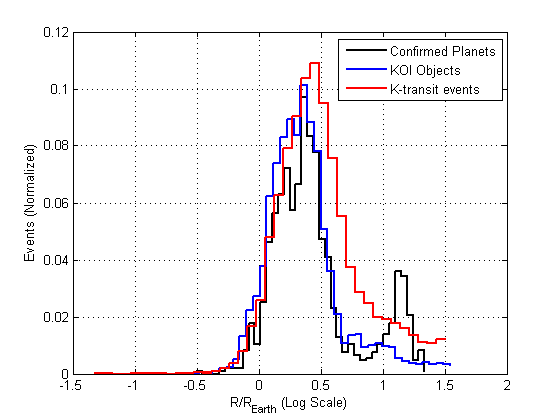
\includegraphics[width=1\columnwidth]{Radius_EventsNormalized} 
\caption[Kepler Events]{Normalized Histogram of Confirmed Exoplanets, Candidate, and Transit Event radius on a log scale $R_{E}=0$ .}
\label{fig:events} 
\end{figure}
Looking at the range $\log{R}=0.4 - 1$ a 2-sample ks-test was preformed on the confirmed planets vs both the candidate and KOI distributions to a significance level of 99\%. The Confirmed planets and Transit events do not come from the same distribution at this significance. The null hypothesis for confirmed and candidate planets can not be rejected at the 99% level. It can be rejected at the 90% level, however. 

%----------------------------------------------------------------------------------------
%	RESULTS AND DISCUSSION
%----------------------------------------------------------------------------------------

\section{Conclusion}
Based on the analysis in section 3, there is a 15 to 20% chance that sub-Jupiture radii objects are under-reported in the confirmed exoplanet database. Reasons for this may stem from the fact that much of the excitement regarding Kepler planets deals with how Earth-like they are. There is a huge area of research devoted to finding a Earth analogue, and describing such a planet. Therefore, much of the exoplanet discovery pipeline is devoted to confirming planets around Earth and Super Earth size. If this is the case then it could impede the scientific communities progress in developing accurate solar system formation models. Such models will eventually put strong constraints on how Earth like planets could form, and where to look for them. Thus, the two objectives are not mutually exclusive. 
The suggestion that Neptune sized planets are being under-represented in the confirmed database is strongly correlated to the assumptions made in section 2.2. Follow-up analysis to ensure that these assumptions are well warranted is the goal of future work. 

%----------------------------------------------------------------------------------------
%	BIBLIOGRAPHY
%----------------------------------------------------------------------------------------

\renewcommand{\refname}{\spacedlowsmallcaps{References}} % For modifying the bibliography heading

\bibliographystyle{plain}
%\bibliographystyle{apa}

\bibliography{DocumentR} % The file containing the bibliography

%----------------------------------------------------------------------------------------

\end{document}